%!TEX root = ../thesis.tex

%TC:ignore
\chapter{Supplementary Figures}

\begin{figure}[p]
\centering
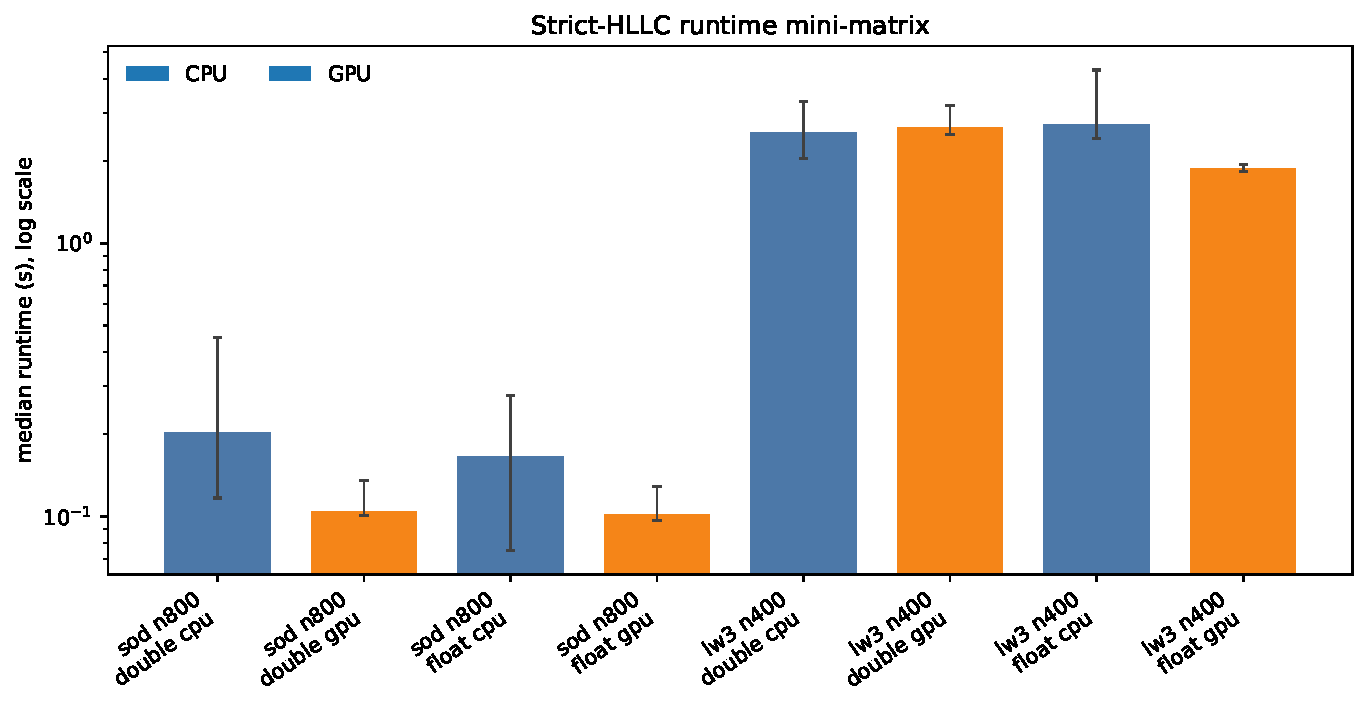
\includegraphics[width=\textwidth]{Figs/report1/appendix_runtime_minimatrix}
\caption[Strict-HLLC runtime mini-matrix]{Strict-HLLC runtime mini-matrix across the matched-binary cases. Bars give wall-clock seconds for the local i9-13900H CPU and the matched CUDA path on the available GPUs (RTX 4060 Laptop locally, RTX 5090 on CSC for Toro3 and Toro5). Non-zero CUDA runtimes confirm that the GPU path is exercised in the comparisons reported in Table~\ref{tab:ch5-cpu-gpu}; the table's zero-drift result is therefore a property of the matched strict-IEEE binary, not of an inactive device.}
\label{fig:app-runtime-minimatrix}
\end{figure}

\begin{figure}[p]
\centering
\begin{subfigure}{0.9\textwidth}
\centering
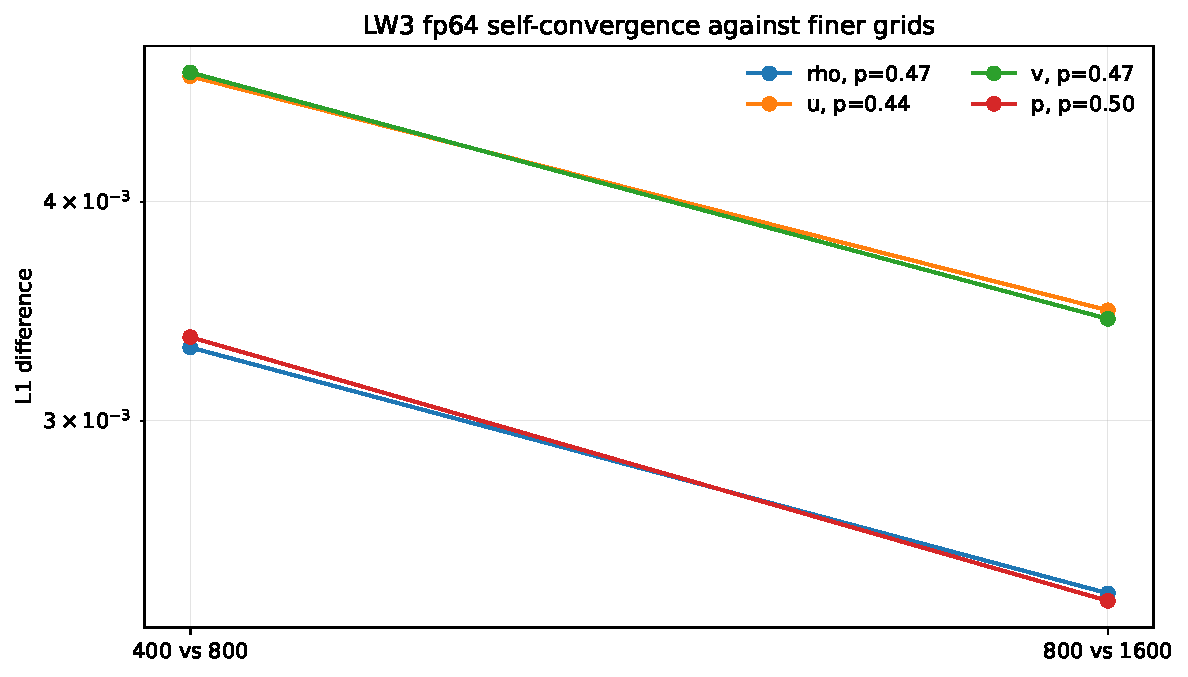
\includegraphics[width=\textwidth]{Figs/report1/appendix_lw3_self_convergence}
\caption{LW3 density self-convergence.}
\label{fig:app-lw3-self-convergence}
\end{subfigure}

\vspace{0.6em}

\begin{subfigure}{0.9\textwidth}
\centering
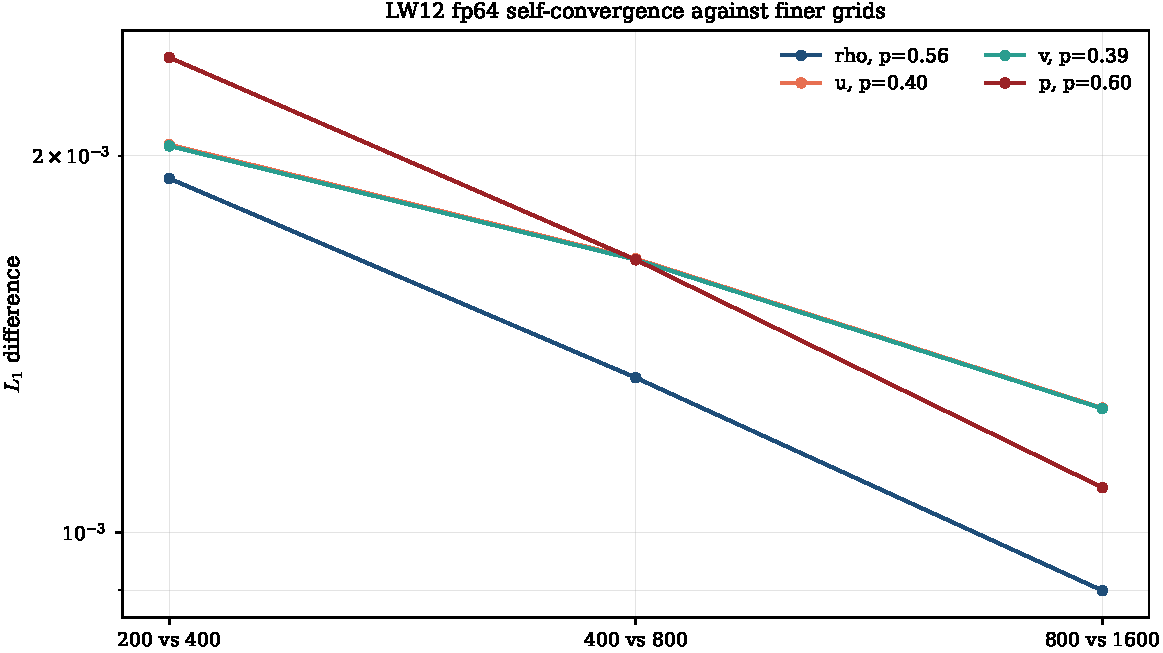
\includegraphics[width=\textwidth]{Figs/report1/appendix_lw12_self_convergence}
\caption{LW12 primitive-variable self-convergence.}
\label{fig:app-lw12-self-convergence}
\end{subfigure}
\caption[LW fp64 self-convergence against finer grids]{LW fp64 self-convergence against finer grids. Panel (a) shows LW3 density $L_1$ between successive grid pairs ($400$ vs $800$, $800$ vs $1600$), with a fitted order of about $0.47$. Panel (b) shows LW12 primitive-variable $L_1$ differences between successive grid pairs ($200$ vs $400$, $400$ vs $800$, $800$ vs $1600$) after block-averaging the finer grid to the coarser. The slow sub-quadratic behaviour supports treating the fine fp64 fields as numerical references rather than exact-solution comparators.}
\label{fig:app-lw-self-convergence}
\end{figure}

\begin{figure}[p]
\centering
\begin{subfigure}{0.96\textwidth}
\centering
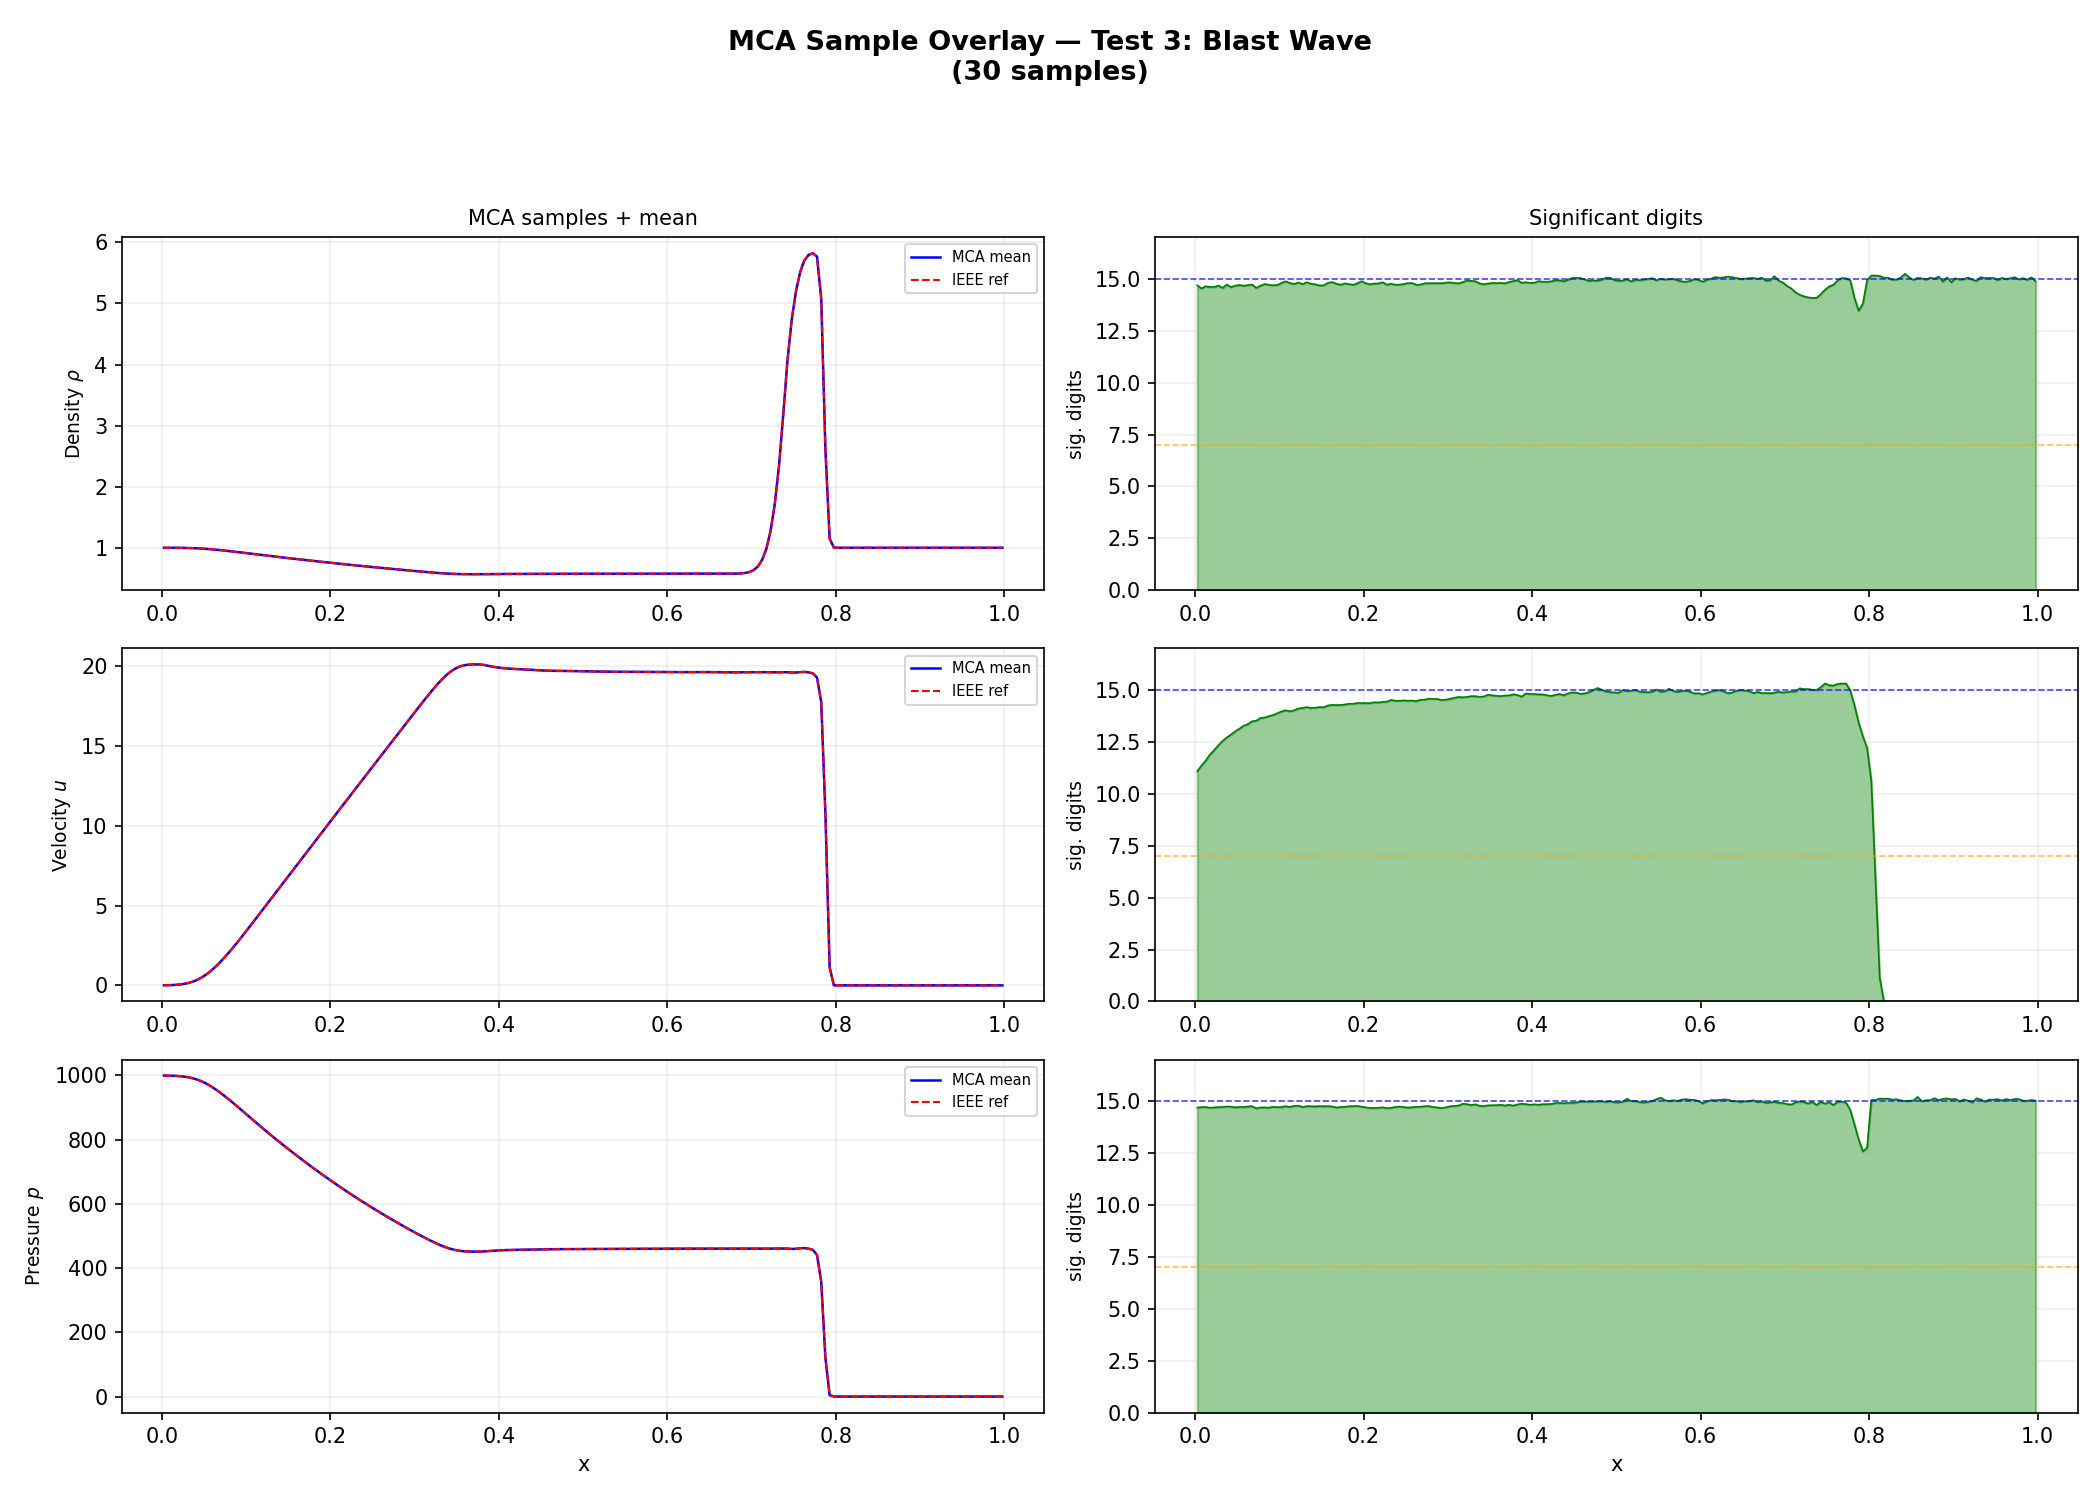
\includegraphics[width=\textwidth,height=0.36\textheight,keepaspectratio]{Figs/report1/appendix_vfc_toro3_overlay}
\caption{MCA sample overlay.}
\end{subfigure}

\vspace{0.5em}

\begin{subfigure}{0.96\textwidth}
\centering
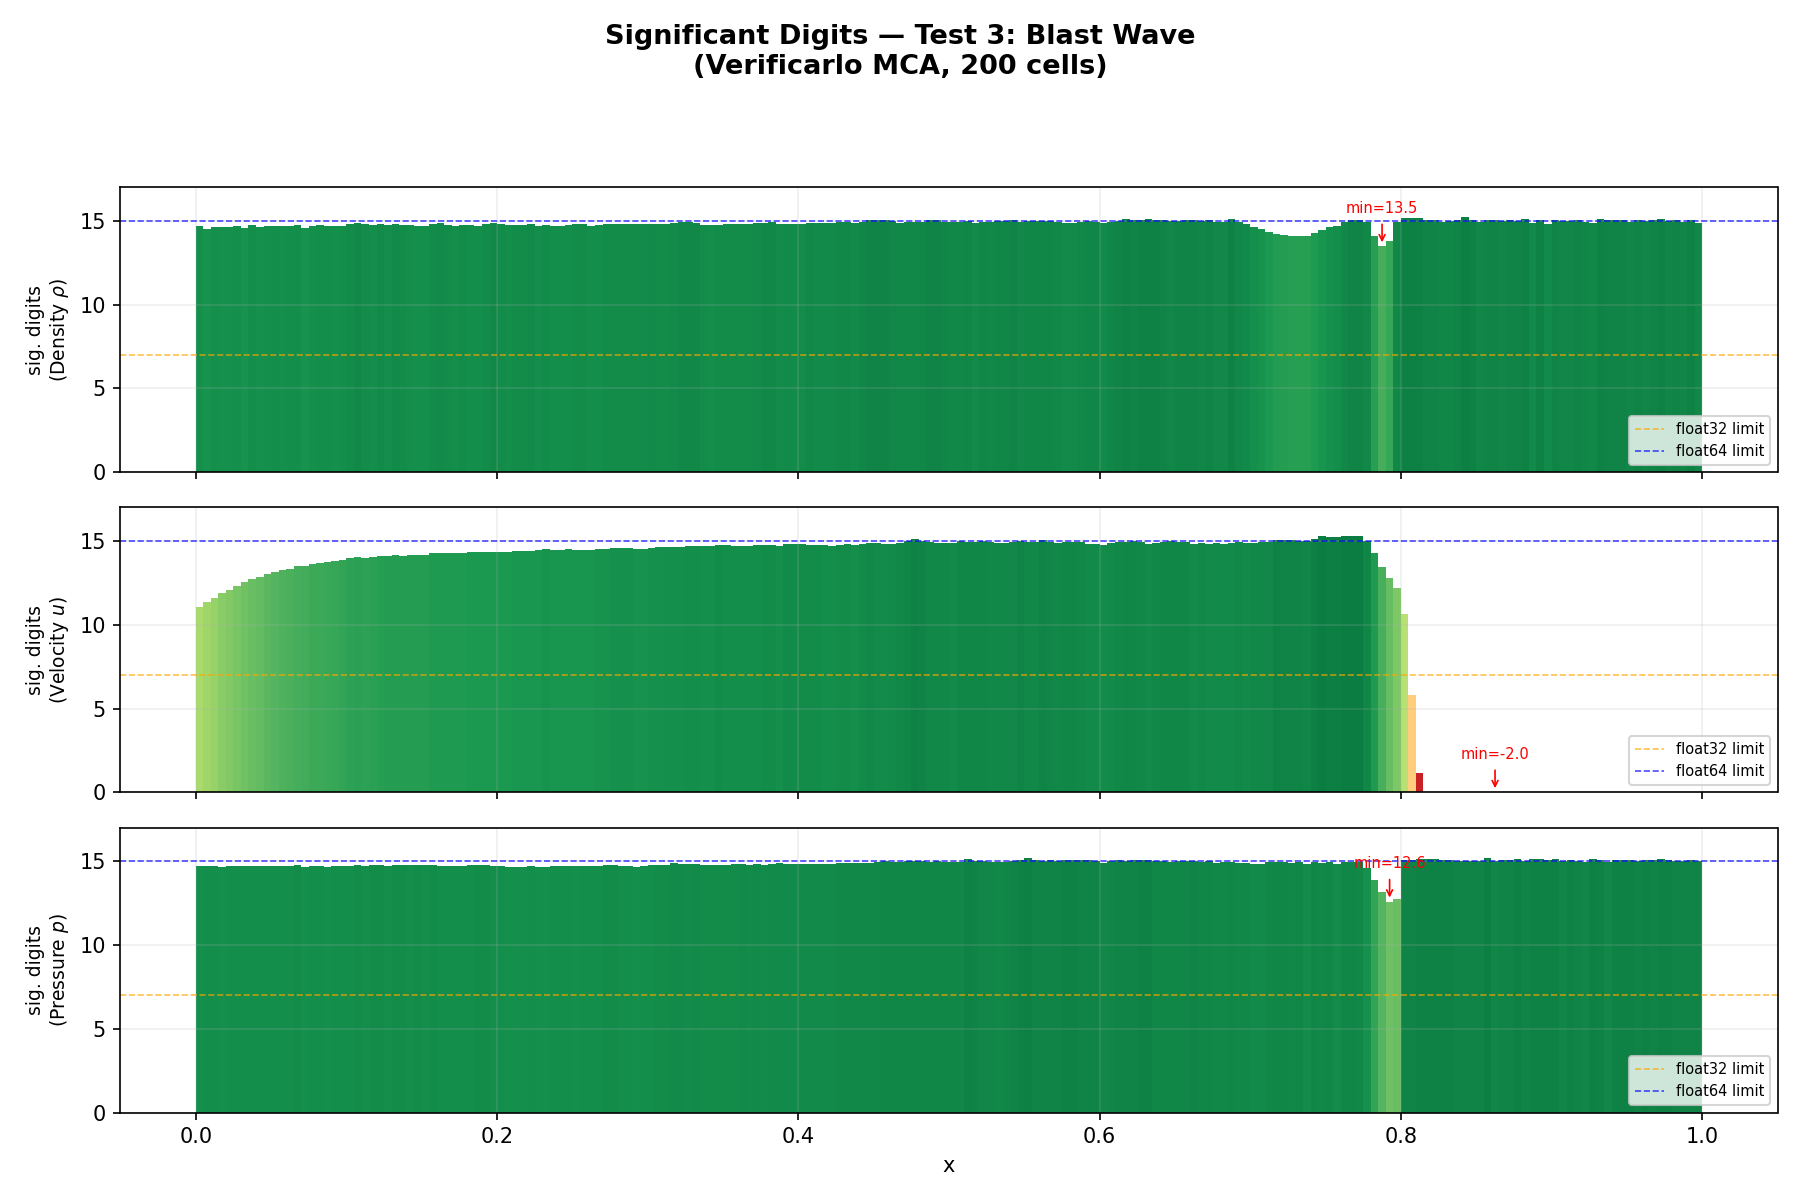
\includegraphics[width=\textwidth,height=0.36\textheight,keepaspectratio]{Figs/report1/appendix_vfc_toro3_heatmap}
\caption{Significant-digit heatmap.}
\end{subfigure}
\caption[Verificarlo MCA diagnostics for Toro3]{Verificarlo MCA stochastic-rounding diagnostics for Toro3 at $N=200$. Panel (a) compares the MCA mean with the IEEE reference for density, velocity, and pressure, and panel (b) maps the corresponding significant-digit structure.}
\label{fig:app-vfc-toro3-diagnostics}
\end{figure}

\begin{figure}[p]\ContinuedFloat
\centering
\begin{subfigure}{0.96\textwidth}
\centering
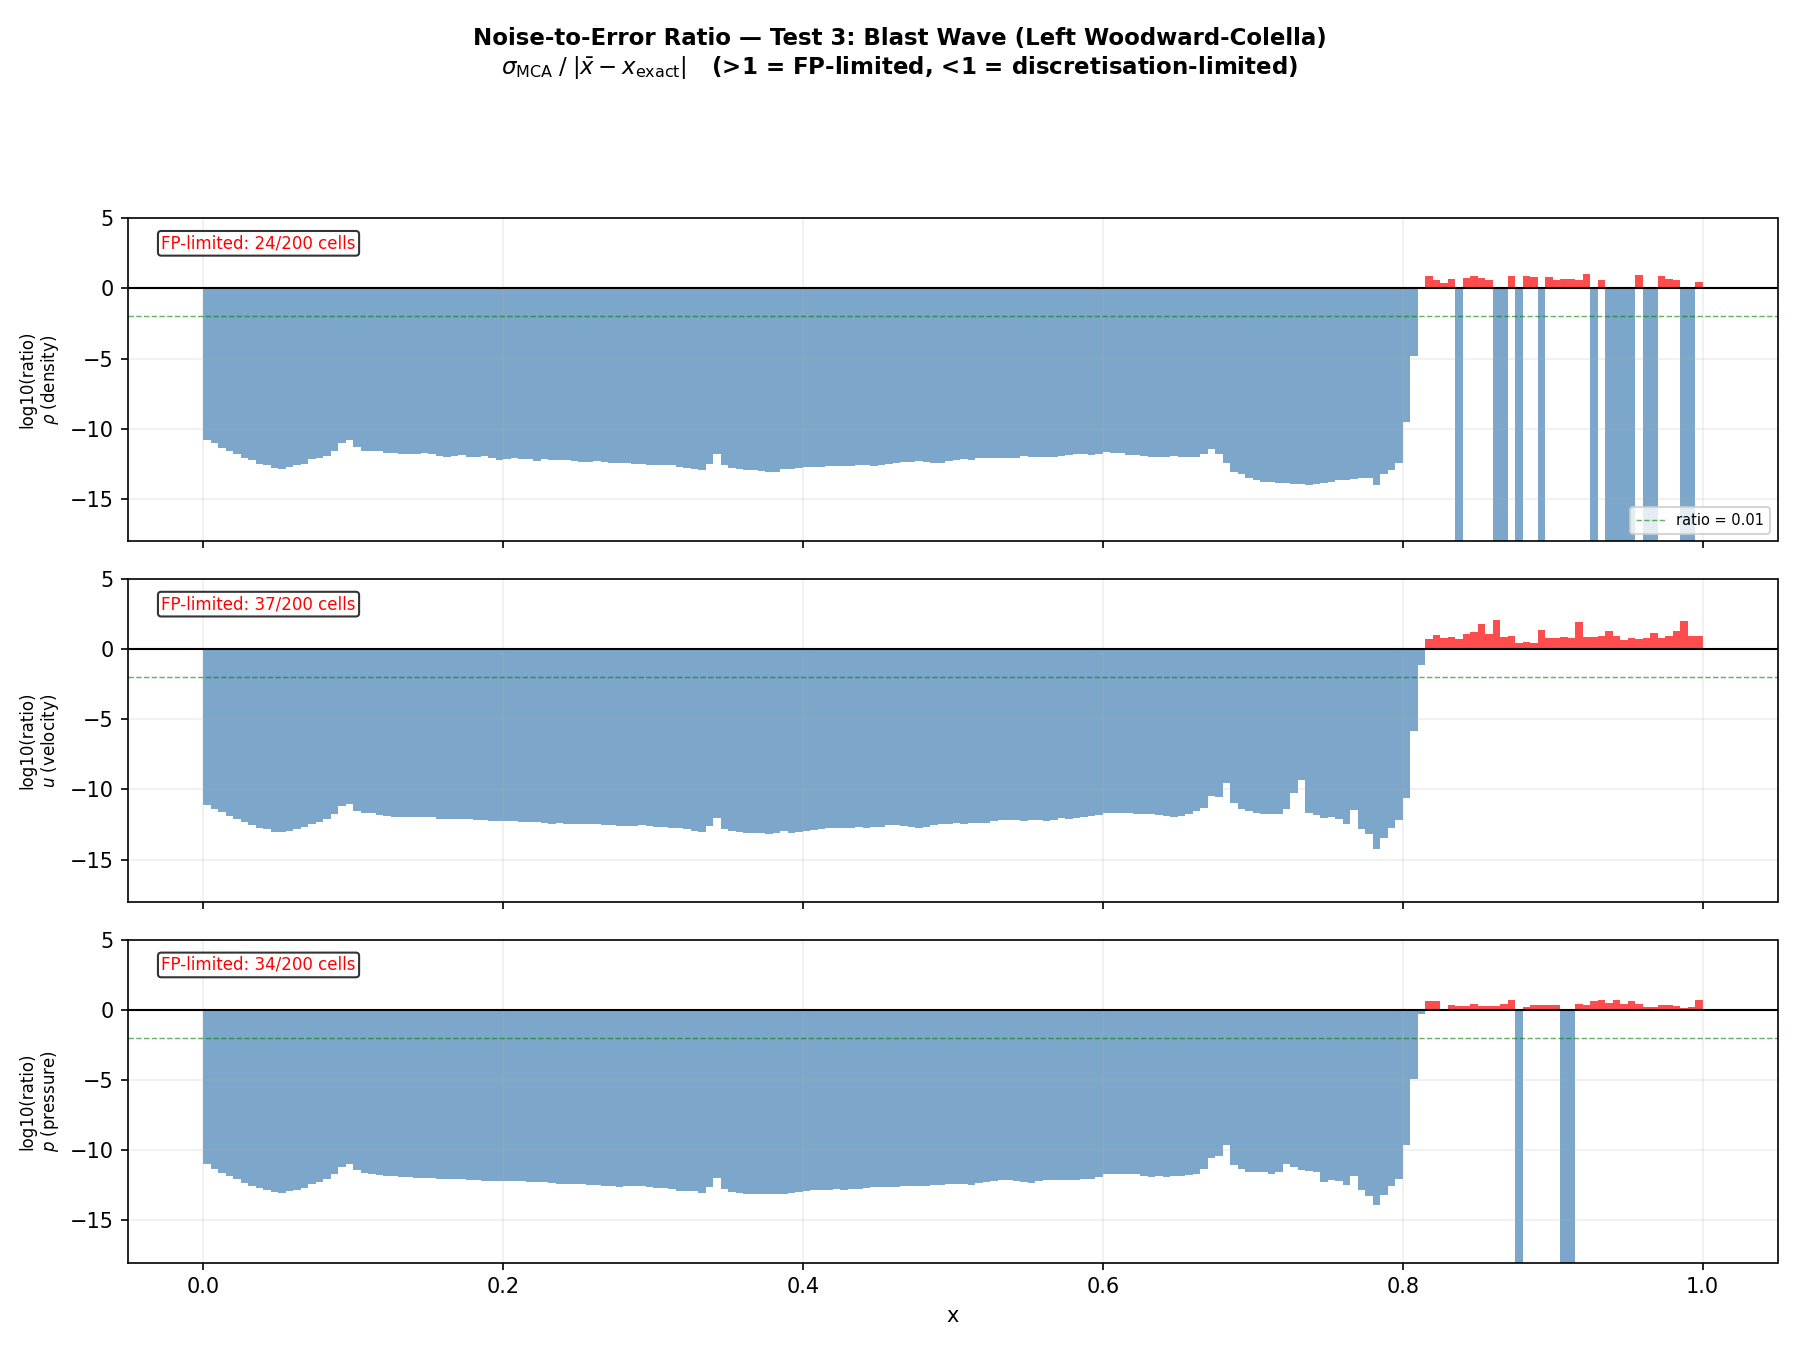
\includegraphics[width=\textwidth,height=0.36\textheight,keepaspectratio]{Figs/report1/appendix_vfc_toro3_noise_ratio}
\caption{Noise-to-error ratio.}
\end{subfigure}

\vspace{0.5em}

\begin{subfigure}{0.96\textwidth}
\centering
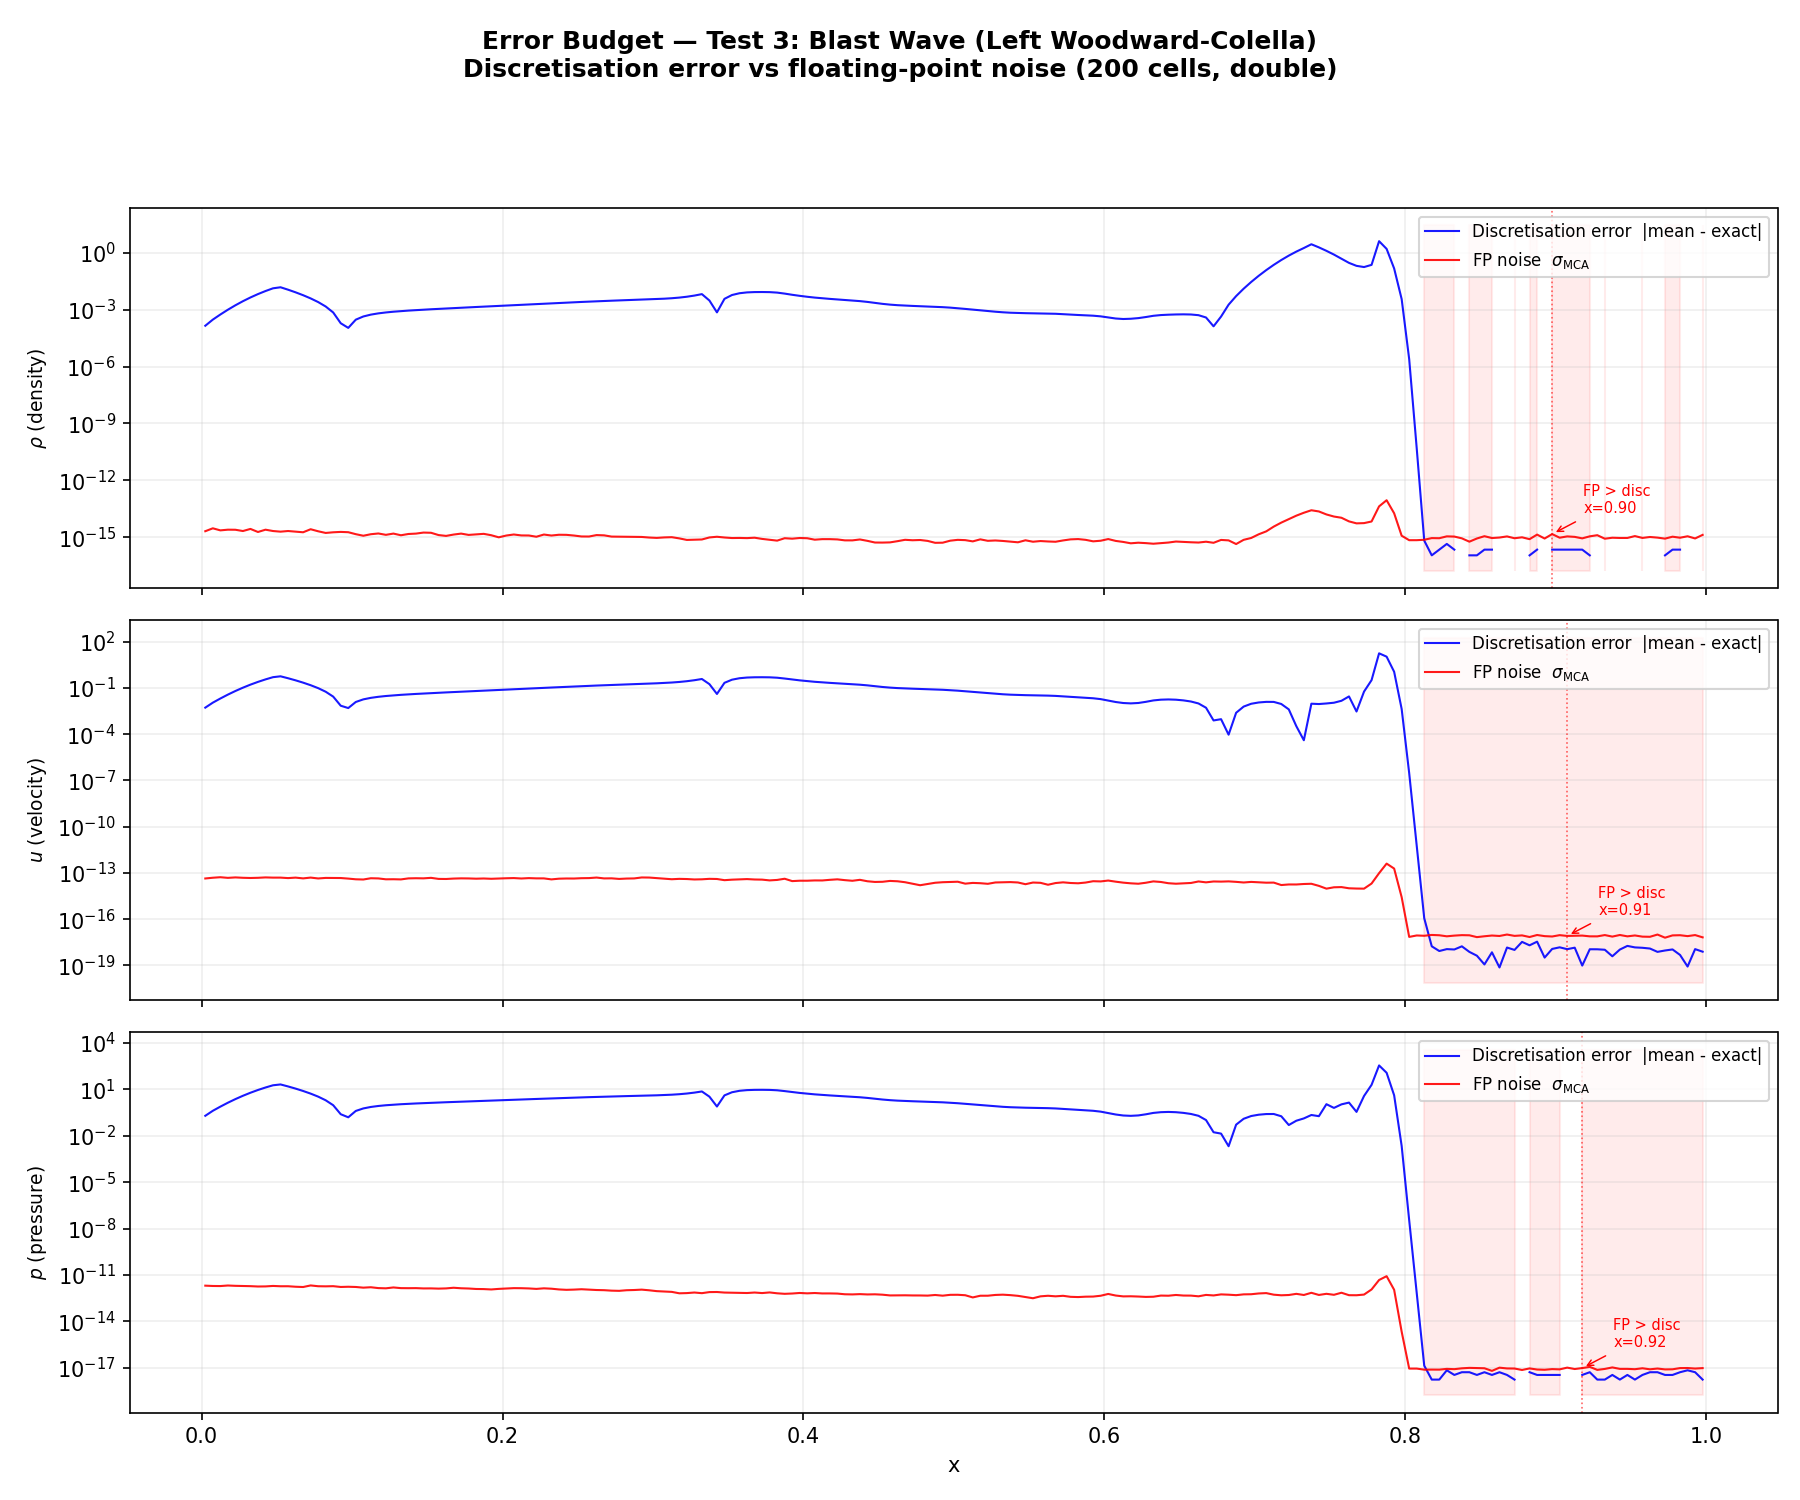
\includegraphics[width=\textwidth,height=0.36\textheight,keepaspectratio]{Figs/report1/appendix_vfc_toro3_error_budget}
\caption{Error-budget view.}
\end{subfigure}
\caption[]{Verificarlo MCA diagnostics for Toro3, continued. Panels (c) and (d) summarize the stochastic-rounding spread relative to reference-scale error. The deterministic fp32 result sits inside the MCA fp32 distribution, indicating that it is not an isolated rounding instance; the fp64 spread is several orders of magnitude tighter, consistent with the precision-scale summary in Table~\ref{tab:ch5-1d-summary}.}
\end{figure}
%TC:endignore
